\documentclass[crop,tikz]{standalone}
\usepackage[utf8]{inputenc}
\usepackage{tikz}
\usepackage{pgfplots}
\usepackage{bm}
\pgfplotsset{compat=newest}
\usepgfplotslibrary{groupplots}
\begin{document}
% This file was created by tikzplotlib v0.8.2.
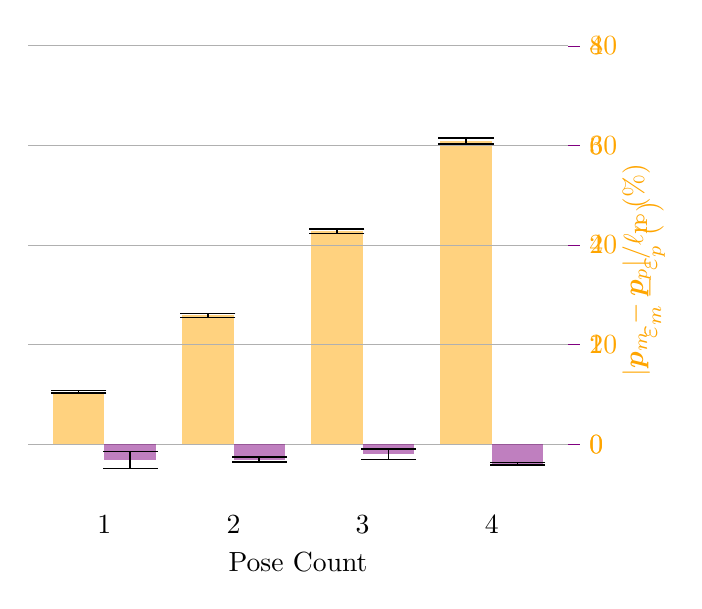
\begin{tikzpicture}
\definecolor{color0}{rgb}{1,0.647058823529412,0}
\definecolor{color1}{rgb}{0.501960784313725,0,0.501960784313725}
\begin{axis}[
anchor=origin,
axis line style={draw=none},
tick align=outside,
tick pos=both,
x grid style={white!69.01960784313725!black},
xmin=-0.59, xmax=3.59,
xtick style={color=black},
xtick style={draw=none},
xtick={0,1,2,3},
xticklabels={ , , , },
y grid style={white!69.01960784313725!black},
ylabel style={color=color0},
ylabel={\(\displaystyle |\bm{p}_m - \bm{p}_p|/\ell_{\textnormal{n}}\) (\%)},
ymin=-0.5, ymax=4,
ytick pos=left,
ytick pos=right,
ytick style={color=color0},
ytick style={color=color0},
yticklabel style={color=color0}
]
\draw[fill=color0,draw opacity=0,fill opacity=0.5] (axis cs:0,0) rectangle (axis cs:-0.4,0.529238963761623);
\draw[fill=color0,draw opacity=0,fill opacity=0.5] (axis cs:1,0) rectangle (axis cs:0.6,1.29410557521853);
\draw[fill=color0,draw opacity=0,fill opacity=0.5] (axis cs:2,0) rectangle (axis cs:1.6,2.13770401008201);
\draw[fill=color0,draw opacity=0,fill opacity=0.5] (axis cs:3,0) rectangle (axis cs:2.6,3.04618308152816);
\path [draw=black, semithick]
(axis cs:-0.2,0.517493718683534)
--(axis cs:-0.2,0.540984208839712);
\path [draw=black, semithick]
(axis cs:0.8,1.27389181483634)
--(axis cs:0.8,1.31431933560072);
\path [draw=black, semithick]
(axis cs:1.8,2.1148891907876)
--(axis cs:1.8,2.16051882937642);
\path [draw=black, semithick]
(axis cs:2.8,3.01677759703155)
--(axis cs:2.8,3.07558856602476);
\addplot [semithick, black, mark=-, mark size=10, mark options={solid}, only marks]
table {%
-0.2 0.517493718683534
0.8 1.27389181483634
1.8 2.1148891907876
2.8 3.01677759703155
};
\addplot [semithick, black, mark=-, mark size=10, mark options={solid}, only marks]
table {%
-0.2 0.540984208839712
0.8 1.31431933560072
1.8 2.16051882937642
2.8 3.07558856602476
};
\end{axis}
\begin{axis}[
anchor=origin,
axis line style={draw=none},
axis y line=right,
tick align=outside,
tick pos=both,
x grid style={white!69.01960784313725!black},
xlabel={Pose Count},
xmin=-0.59, xmax=3.59,
xtick style={color=black},
xtick style={draw=none},
xtick={0,1,2,3},
xticklabels={1,2,3,4},
y grid style={white!69.01960784313725!black},
ylabel style={color=color0},
ylabel={\(\displaystyle \varepsilon_m - \varepsilon_p\) (\(\displaystyle ^\circ\))},
ymajorgrids,
ymin=-10, ymax=80,
ytick pos=left,
ytick pos=right,
ytick style={color=color0},
ytick style={color=color1},
yticklabel style={color=color0}
]
\draw[fill=color1,draw opacity=0,fill opacity=0.5] (axis cs:0,0) rectangle (axis cs:0.4,-3.15611166460704);
\draw[fill=color1,draw opacity=0,fill opacity=0.5] (axis cs:1,0) rectangle (axis cs:1.4,-3.05345326636424);
\draw[fill=color1,draw opacity=0,fill opacity=0.5] (axis cs:2,0) rectangle (axis cs:2.4,-2.00026514436573);
\draw[fill=color1,draw opacity=0,fill opacity=0.5] (axis cs:3,0) rectangle (axis cs:3.4,-3.89494743878987);
\path [draw=black, semithick]
(axis cs:0.2,-1.42888978396942)
--(axis cs:0.2,-4.88333354524465);
\path [draw=black, semithick]
(axis cs:1.2,-2.60250926153842)
--(axis cs:1.2,-3.50439727119007);
\path [draw=black, semithick]
(axis cs:2.2,-0.946153478876033)
--(axis cs:2.2,-3.05437680985542);
\path [draw=black, semithick]
(axis cs:3.2,-3.64376902645675)
--(axis cs:3.2,-4.14612585112299);
\addplot [semithick, black, mark=-, mark size=10, mark options={solid}, only marks]
table {%
0.2 -1.42888978396942
1.2 -2.60250926153842
2.2 -0.946153478876033
3.2 -3.64376902645675
};
\addplot [semithick, black, mark=-, mark size=10, mark options={solid}, only marks]
table {%
0.2 -4.88333354524465
1.2 -3.50439727119007
2.2 -3.05437680985542
3.2 -4.14612585112299
};
\end{axis}
\end{tikzpicture}
%% End matplotlib2tikz content %% 
\end{document}